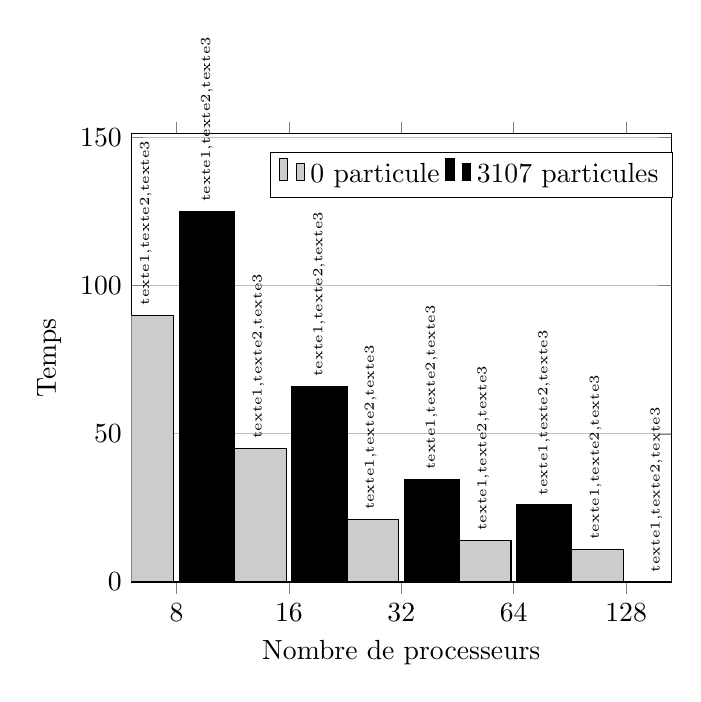
\begin{tikzpicture} \begin{axis}[
    x tick label style={
        /pgf/number format/1000 sep=},
    ymajorgrids,
    ylabel=Temps,
    xlabel= Nombre de processeurs,
    nodes near coords={texte1,texte2,texte3},
    xtick={1,2,3,4,5},
    xticklabels={$8$,$16$,$32$,$64$,$128$},
    enlarge y limits={upper,value=0.21},
    legend style={at={(0.63,0.96)},
        anchor=north,legend columns=-1},
    ybar,
    every node near coord/.append style={rotate=90, anchor=west,font=\tiny},
    bar width=20pt,
]
\addplot [ybar,fill=gray!40]
    coordinates {(1,90) (2,45)
         (3,21) (4,14) (5,11)};
\addplot [ybar,fill=black]
    coordinates {(1,125) (2,66)
        (3,34.5) (4,26) (5,0)};
\legend{0 particule,3107 particules,temps th\'eorique}
\end{axis}
\end{tikzpicture}
